% !TeX spellcheck = es_ES
% !TEX encoding = UTF-8 Unicode
\documentclass[t, compress, spanish, aspectratio=169]{beamer}
%\documentclass[handout]{beamer}    % for the handout

\usetheme[progressbar=frametitle]{metropolis}

\setbeamertemplate{navigation symbols}{} % Gets rid of navigation symbols

\usepackage{dsfont} % Double stroke fonts for math symbols
\usepackage[english]{babel} % Manages differences between languages: hyphenation etc

\usepackage{appendixnumberbeamer} % Does not include backup slides in the number of pages

\usepackage{centernot} % To draw not in math symbols (does not imply)

\usepackage{ragged2e}  % Text alignment
\justifying

\usepackage{graphicx} % Format for graphics: additional options for includefigure
\usepackage{pgf} % Tool for graphics

\usepackage{booktabs} % Format for tables: top, bottom and mid lines
\usepackage[scale=2]{ccicons}
\usepackage{threeparttable} % Format for tables
\usepackage{lscape} % Landscape for tables

% Customized commands
  \newcommand{\vs}{\vskip0pt plus.5fill}
  \newcommand{\SR}{\mathbb{R}}
  \DeclareMathOperator{\plim}{plim}
  \DeclareMathOperator{\Var}{Var}
  \DeclareMathOperator{\Avar}{AVar}
  \DeclareMathOperator{\Cov}{Cov}
  \DeclareMathOperator{\N}{Normal}
  \DeclareMathOperator{\E}{\mathbb{E}}
  \DeclareMathOperator{\LP}{\mathbb{L}}
  \newcommand{\pto}{\stackrel{p}{\longrightarrow}}
  \newcommand{\dto}{\stackrel{d}{\longrightarrow}}
  \newcommand{\adistr}{\stackrel{a}{\sim}}
  \newcommand{\epsi}{\varepsilon}
  \newcommand\independent{\protect\mathpalette{\protect\independenT}{\perp}}
  \def\independenT#1#2{\mathrel{\rlap{$#1#2$}\mkern2mu{#1#2}}}
  \newcommand{\term}[1]{\structure{\textbf{#1}}} % label/definition markup, distinct from \alert (reserved for genuine callouts)


\title [Discriminaci\'on] {An\'alisis Econom\'etrico\\
	Discriminaci\'on en el mercado laboral:\\ experimento vs. datos observacionales}
\author[de Elejalde]{Ramiro de Elejalde}
\institute [UAH] {Facultad de Econom\'ia y Finanzas \\ Universidad Alberto Hurtado}
\date[\today] {}
\subject{An\'alisis Econom\'etrico}
\begin{document}

	%------------------------------------------------------------

	\begin{frame}
		\titlepage
	\end{frame}

	% --------------------------------------------------- Slide --
	\begin{frame}
		\frametitle{Outline}
		\footnotesize
		\tableofcontents
		\alert{Referencias}: Bertrand y Mullainathan (2004, AER); cap. 3.2.2 de Angrist and Pischke; secci\'on de sesgo de variable omitida de la clase 4.
	\end{frame}

	% ============================================================
	\section{La pregunta y el problema de identificaci\'on}
	% ============================================================

	% --------------------------------------------------- Slide --
	\begin{frame}
		\frametitle{?`C\'omo se mide la discriminaci\'on en el mercado laboral?}
		\begin{itemize}
			\item \term{Pregunta}: ?`Dos personas con las mismas calificaciones reciben el mismo trato en el mercado laboral, independientemente de su raza?
			\item El dato crudo es conocido: en Estados Unidos la tasa de empleo de la poblaci\'on negra es sistem\'aticamente menor que la de la poblaci\'on blanca.
			\item \alert{Pero una brecha no es un efecto.} La brecha mezcla trato desigual con todo lo dem\'as que difiere entre los dos grupos: educaci\'on, experiencia, redes de contactos, lugar de residencia.
			\item \term{El problema}: la raza no se asigna al azar. Nunca observamos a la misma persona en los dos estados.
		\end{itemize}
	\end{frame}

	% --------------------------------------------------- Slide --
	\begin{frame}
		\frametitle{Dos estrategias, la misma regresi\'on}
		\small
		\begin{itemize}
			\item Vamos a estimar \alert{dos veces la misma ecuaci\'on}:
			\begin{align*}
				y_i = \beta_0 + \beta_1 \, negro_i + \gamma' x_i + u_i
			\end{align*}
			con $y_i$ binaria, $negro_i$ una dummy y $x_i$ una lista de controles que iremos agrandando.
			\item \term{Parte A --- Experimento}: Bertrand y Mullainathan (2004) mandaron currículos ficticios a avisos reales, asignando el \alert{nombre al azar}. $y_i$: la empresa llam\'o para entrevista.
			\item \term{Parte B --- Datos observacionales}: CPS 2024 (encuesta de hogares de EE.UU.). $y_i$: la persona est\'a empleada.
			\item \alert{La ecuaci\'on es id\'entica. La interpretaci\'on no lo es en absoluto.}
			\item [] La pregunta que organiza toda la clase: \term{?`qu\'e le pasa a $\hat\beta_1$ cuando agregamos controles?}
		\end{itemize}
	\end{frame}

	% ============================================================
	\section{Parte A: el experimento de curr\'iculos}
	% ============================================================

	% --------------------------------------------------- Slide --
	\begin{frame}
		\frametitle{El dise\~no de Bertrand y Mullainathan (2004)}
		\small
		\begin{itemize}
			\item \term{Idea}: mandar curr\'iculos ficticios a avisos de trabajo \alert{reales} y medir a qui\'en llaman.
			\item \term{Muestra}: 4.870 curr\'iculos enviados a avisos de ventas y apoyo administrativo publicados en diarios de Boston y Chicago (2001--2002).
			\item \term{El tratamiento}: a cada curr\'iculo se le asign\'o \alert{al azar} un nombre
			\begin{itemize}
				\item t\'ipicamente blanco: Emily Walsh, Greg Baker, \ldots
				\item t\'ipicamente afroamericano: Lakisha Washington, Jamal Jones, \ldots
			\end{itemize}
			\item \term{Variable dependiente}: $callback_i = 1$ si la empresa llam\'o para una entrevista.
			\item [] \alert{Lo \'unico que cambia entre un curr\'iculo y otro es el nombre.} Todo lo dem\'as --- experiencia, educaci\'on, habilidades --- se sorte\'o de forma independiente del nombre.
		\end{itemize}
	\end{frame}

	% --------------------------------------------------- Slide --
	\begin{frame}
		\frametitle{?`Funcion\'o la aleatorizaci\'on? Tabla de balance}
		\scriptsize
		\begin{center}
			
\begin{tabular}[t]{lrrrr}
\toprule
Variable & Nombre blanco & Nombre afroamericano & Diferencia & Error estándar\\
\midrule
Años de experiencia & 7.856 & 7.830 & -0.027 & 0.145\\
Cantidad de empleos previos & 3.664 & 3.658 & -0.006 & 0.035\\
Currículo de alta calidad & 0.502 & 0.502 & 0.000 & 0.014\\
Tiene distinciones & 0.054 & 0.051 & -0.003 & 0.006\\
Trabajo voluntario & 0.409 & 0.414 & 0.006 & 0.014\\
Servicio militar & 0.092 & 0.102 & 0.009 & 0.008\\
Huecos en el historial & 0.450 & 0.446 & -0.004 & 0.014\\
Sabe computación & 0.809 & 0.832 & 0.024 & 0.011\\
Algo de universidad & 0.716 & 0.723 & 0.007 & 0.013\\
Mujer & 0.764 & 0.775 & 0.011 & 0.012\\
Chicago (vs. Boston) & 0.555 & 0.555 & 0.000 & 0.014\\
\bottomrule
\end{tabular}

		\end{center}
		\vspace{-0.2cm}
		Las once diferencias son chicas y ninguna supera dos errores est\'andar. \term{Los dos grupos de curr\'iculos son iguales en todo menos en el nombre.}
	\end{frame}

	% --------------------------------------------------- Slide --
	\begin{frame}
		\frametitle{Resultado crudo: tasa de llamados}
		\begin{center}
			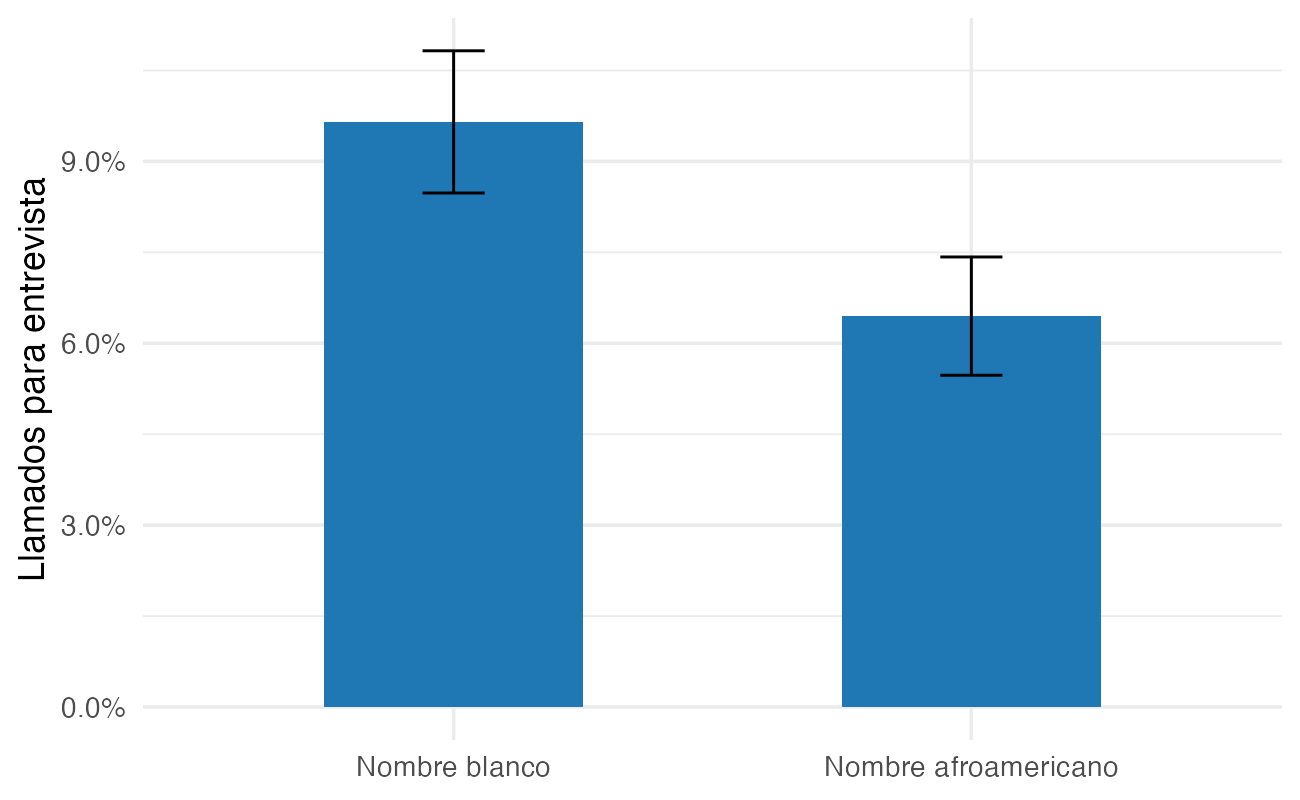
\includegraphics[width=0.62\textwidth]{figures/callback_rates.png}
		\end{center}
		\vspace{-0.2cm}
		\small 9.65\% con nombre blanco contra 6.45\% con nombre afroamericano: \term{una brecha de 3.2 puntos porcentuales}. Un curr\'iculo con nombre blanco necesita mandar unas 10 postulaciones para conseguir un llamado; con nombre afroamericano, unas 15.
	\end{frame}

	% --------------------------------------------------- Slide --
	\begin{frame}
		\frametitle{La ecuaci\'on emp\'irica}
		\small
		\begin{itemize}
			\item []
			\begin{align*}
				callback_i = \beta_0 + \beta_1 \, negro_i + \gamma' x_i + u_i
			\end{align*}
			\item \term{Modelo de probabilidad lineal}: la variable dependiente es binaria, as\'i que $\E(callback_i | negro_i, x_i)$ es una \alert{probabilidad}, y $\beta_1$ se lee como cambio en la probabilidad de recibir un llamado.
			\item \term{Identificaci\'on}: el nombre se asign\'o al azar, entonces
			\begin{align*}
				negro_i \independent (u_i, x_i) \quad \Longrightarrow \quad \E(u_i | negro_i) = 0 \ \text{ \alert{por dise\~no}}.
			\end{align*}
			\item [] No es un supuesto que tengamos que defender con argumentos: lo garantiza el sorteo.
			\item \term{Predicci\'on}: si esto es cierto, \alert{agregar controles no deber\'ia mover $\hat\beta_1$.}
		\end{itemize}
	\end{frame}

	% --------------------------------------------------- Slide --
	\begin{frame}
		\frametitle{Estimaci\'on: ?`se mueve el coeficiente?}
		\footnotesize
		\begin{center}
			\begin{table}
\centering
\begin{tabular}[t]{lcccc}
\toprule
  & (1) Sin controles & (2) + Ciudad, sexo & (3) + Currículo & (4) + Industria\\
\midrule
Nombre afroamericano & -0.0320 & -0.0322 & -0.0313 & -0.0312\\
 & (0.0078) & (0.0078) & (0.0077) & (0.0077)\\
\midrule
Num.Obs. & 4,870 & 4,870 & 4,870 & 4,870\\
R2 & 0.003 & 0.007 & 0.030 & 0.033\\
\bottomrule
\end{tabular}
\end{table}

		\end{center}
		\vspace{-0.1cm}
		Controles: (2) ciudad y sexo; (3) las quince caracter\'isticas del curr\'iculo (experiencia, empleos previos, calidad, distinciones, voluntariado, servicio militar, huecos en el historial, computaci\'on, universidad, \ldots); (4) efectos fijos de industria del aviso. Errores est\'andar robustos (HC1).
	\end{frame}

	% --------------------------------------------------- Slide --
	\begin{frame}
		\frametitle{El coeficiente no se mueve}
		\small
		\begin{itemize}
			\item De $-0.0320$ a $-0.0312$: \alert{un movimiento de 2.5\%}, muy adentro de un error est\'andar.
			\item \term{Esto es exactamente lo que predice la teor\'ia.} Con asignaci\'on al azar, los controles son ortogonales al tratamiento: sacarlos no genera sesgo.
			\item ?`Para qu\'e sirven entonces los controles ac\'a? Para \term{ganar precisi\'on}: explican parte de $u_i$ y reducen la varianza residual. El $R^2$ sube de 0.003 a 0.033.
			\item [] (En este caso la ganancia de precisi\'on es chica: el error est\'andar baja de 0.0078 a 0.0077.)
			\item \alert{Cuando la estimaci\'on es cre\'ible, la tabla de robustez es aburrida. Eso es una buena se\~nal, no una mala.}
		\end{itemize}
	\end{frame}

	% ============================================================
	\section{Parte B: los datos observacionales (CPS 2024)}
	% ============================================================

	% --------------------------------------------------- Slide --
	\begin{frame}
		\frametitle{Ahora sin experimento: CPS 2024}
		\small
		\begin{itemize}
			\item \term{Fuente}: Current Population Survey 2024 (archivo MORG del NBER), la encuesta de hogares de Estados Unidos.
			\item \term{Poblaci\'on}: personas de 22 a 40 a\~nos, blancas o negras no hispanas. $N=46.885$.
			\item [] El rango de edad busca parecerse a la poblaci\'on del experimento: postulantes a empleos de entrada, con pocos a\~nos de experiencia.
			\item \term{Variable dependiente}: $empleado_i = 1$ si la persona est\'a ocupada.
			\item \term{Variable de inter\'es}: $negro_i$.
			\item [] Misma forma de regresi\'on que la Parte A. \alert{Lo \'unico que cambia es que ahora nadie sorte\'o nada.}
		\end{itemize}
	\end{frame}

	% --------------------------------------------------- Slide --
	\begin{frame}
		\frametitle{Estad\'isticas descriptivas por grupo}
		\footnotesize
		\begin{center}
			\begin{table}
\centering
\begin{tabular}[t]{lrr}
\toprule
  & Blanco & Negro\\
\midrule
Empleado & 0.821 & 0.743\\
Mujer & 0.501 & 0.538\\
Edad & 31.537 & 31.202\\
Casado/a & 0.473 & 0.244\\
Vive en área metropolitana & 0.792 & 0.905\\
Universitaria completa o más & 0.461 & 0.305\\
\bottomrule
\end{tabular}
\end{table}

		\end{center}
		\vspace{-0.1cm}
		\small A diferencia de la tabla de balance de la Parte A, ac\'a los dos grupos \alert{difieren en todo}: educaci\'on universitaria (46\% vs. 31\%), estado civil (47\% vs. 24\%), residencia metropolitana (79\% vs. 91\%). \term{Estas diferencias son justamente el problema.}
	\end{frame}

	% --------------------------------------------------- Slide --
	\begin{frame}
		\frametitle{Estimaci\'on: ahora s\'i se mueve}
		\footnotesize
		\begin{center}
			\begin{table}
\centering
\begin{tabular}[t]{lcccc}
\toprule
  & (1) Sin controles & (2) + Sexo, edad & (3) + Educación & (4) + Estado, familia\\
\midrule
Negro & -0.0778 & -0.0729 & -0.0479 & -0.0358\\
 & (0.0058) & (0.0057) & (0.0056) & (0.0059)\\
\midrule
Num.Obs. & 46,885 & 46,885 & 46,885 & 46,885\\
R2 & 0.005 & 0.023 & 0.063 & 0.069\\
\bottomrule
\end{tabular}
\end{table}

		\end{center}
		\vspace{-0.1cm}
		Controles: (2) sexo, edad y edad al cuadrado; (3) cinco categor\'ias de m\'aximo nivel educativo; (4) estado civil, residencia metropolitana y efectos fijos de estado. Errores est\'andar robustos (HC1). \alert{Las cuatro columnas usan la misma muestra.}
	\end{frame}

	% --------------------------------------------------- Slide --
	\begin{frame}
		\frametitle{?`Por qu\'e se mueve? Sesgo de variable omitida}
		\small
		\begin{itemize}
			\item Modelo largo y modelo corto:
			\begin{align*}
				empleado_i &= \beta_0 + \beta_1 \, negro_i + \beta_2 \, educ_i + u_i \quad \text{(largo)}\\
				empleado_i &= \delta_0 + \delta_1 \, negro_i + v_i \quad \text{(corto)}
			\end{align*}
			\item La relaci\'on entre ambos, con $\pi_1$ el coeficiente de $negro_i$ en la regresi\'on auxiliar de $educ_i$ sobre $negro_i$:
			\begin{align*}
				\delta_1 = \beta_1 + \beta_2 \, \pi_1
			\end{align*}
			\item En el CPS: $\pi_1 < 0$ (menos educaci\'on universitaria) y $\beta_2 > 0$ (m\'as educaci\'on, m\'as empleo), entonces \alert{$\beta_2 \pi_1 < 0$}: el modelo corto exagera la brecha.
			\item \term{En la Parte A}, $\pi_1 = 0$ por aleatorizaci\'on $\Rightarrow \delta_1 = \beta_1$. \alert{Esa es toda la diferencia entre los dos ejercicios.}
		\end{itemize}
	\end{frame}

	% ============================================================
	\section{Comparaci\'on: qu\'e aprendimos}
	% ============================================================

	% --------------------------------------------------- Slide --
	\begin{frame}
		\frametitle{Los dos ejercicios, lado a lado}
		\begin{center}
			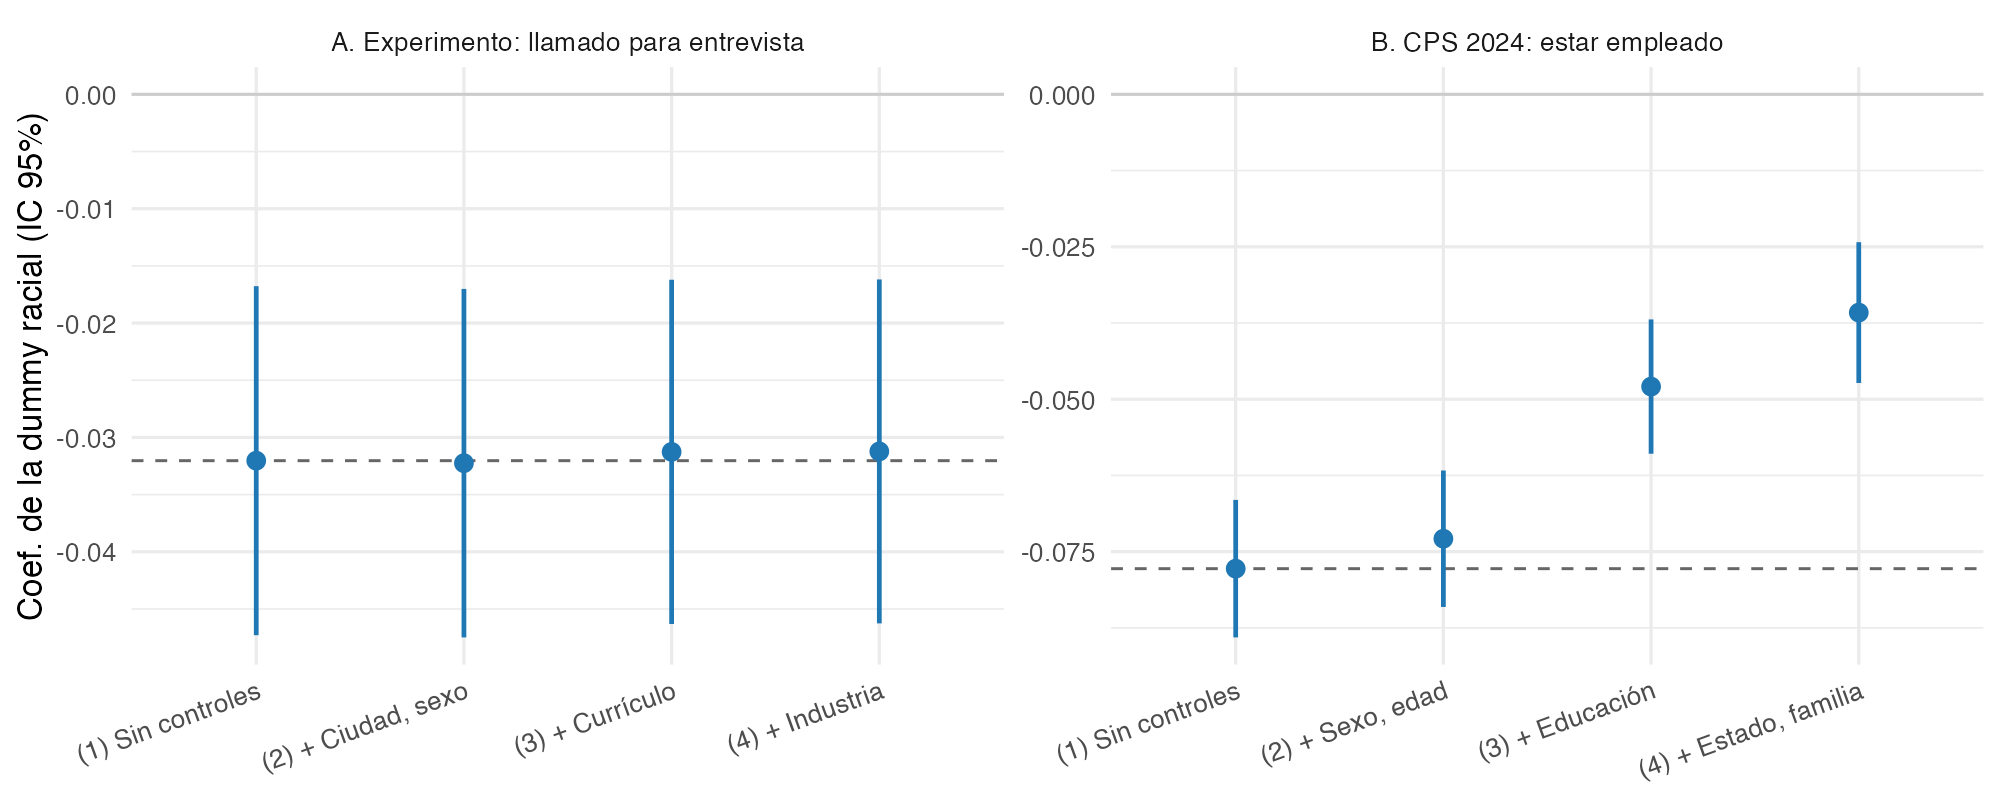
\includegraphics[width=0.95\textwidth]{figures/coef_comparison.png}
		\end{center}
		\vspace{-0.3cm}
		\small La l\'inea punteada marca la estimaci\'on sin controles. \term{Panel A: el coeficiente se queda quieto (2.5\%). Panel B: se mueve 54\%.}
	\end{frame}

	% --------------------------------------------------- Slide --
	\begin{frame}
		\frametitle{?`Y si agregamos m\'as controles?}
		\small
		\begin{itemize}
			\item Tentaci\'on natural: si el coeficiente se mueve, agreguemos controles hasta que se quede quieto.
			\item \alert{No funciona}, por tres razones distintas:
			\begin{enumerate}
				\item \term{Inobservables}: quedan afuera calidad de la escuela, redes de contactos, riqueza familiar, salud. Nada garantiza que lo que falta sea chico.
				\item \term{Malos controles}: la educaci\'on \emph{no} es una variable de fondo. Si la discriminaci\'on reduce los retornos esperados de estudiar, entonces $educ_i$ es en parte un \alert{resultado} de lo que queremos medir. Controlar por ella saca parte del efecto.
				\item \term{Selecci\'on muestral}: estar empleado y ser encuestado no son independientes de la raza. La poblaci\'on encarcelada, por ejemplo, queda fuera del CPS.
			\end{enumerate}
			\item [] \alert{Controlar por m\'as variables no convierte una comparaci\'on observacional en un experimento.}
		\end{itemize}
	\end{frame}

	% --------------------------------------------------- Slide --
	\begin{frame}
		\frametitle{Una coincidencia peligrosa}
		\small
		\begin{itemize}
			\item El modelo (4) del CPS da $-0.0358$. El experimento da $-0.0312$. \alert{Numeros parecidos.}
			\item Es tentador leer eso como que ``los controles funcionaron''. \term{Es una coincidencia}, y compararlos directamente es un error:
			\begin{itemize}
				\item \term{Variable dependiente distinta}: recibir un llamado en una postulaci\'on vs. estar empleado.
				\item \term{Poblaci\'on distinta}: postulantes a empleos de entrada en dos ciudades en 2001 vs. toda la poblaci\'on de 22 a 40 a\~nos de EE.UU. en 2024.
				\item \term{Estimando distinto}: el experimento identifica el efecto de la \emph{percepci\'on} del nombre en la etapa de selecci\'on de curr\'iculos. El CPS mide una \emph{brecha} de empleo.
			\end{itemize}
			\item \alert{Que dos numeros se parezcan no valida el que no est\'a identificado.}
		\end{itemize}
	\end{frame}

	% --------------------------------------------------- Slide --
	\begin{frame}
		\frametitle{Qu\'e mide realmente el experimento}
		\small
		\begin{itemize}
			\item \term{Lo que s\'i}: en la etapa de \alert{screening de curr\'iculos}, para avisos de empleos de entrada en Boston y Chicago, el nombre percibido cambia causalmente la probabilidad de ser llamado.
			\item \term{Lo que no}: no mide discriminaci\'on en salarios, en promociones, ni en la entrevista misma. No mide el efecto de ser una persona negra en el mercado laboral.
			\item \term{Validez externa}: dos ciudades, dos sectores, principios de los 2000. La \alert{validez interna} es impecable; la externa hay que argumentarla aparte.
			\item [] Este es el trade-off cl\'asico: el experimento compra identificaci\'on a costa de acotar mucho la pregunta.
		\end{itemize}
	\end{frame}

	% --------------------------------------------------- Slide --
	\begin{frame}
		\frametitle{Resumen}
		\small
		\begin{itemize}
			\item Corrimos \term{la misma regresi\'on} en dos bases de datos y obtuvimos dos objetos distintos: un \alert{efecto causal} y una \alert{brecha descriptiva}.
			\item Lo que separa a uno del otro no es el estimador, ni la cantidad de controles, ni el $R^2$. Es \alert{c\'omo se gener\'o la variable de inter\'es}.
			\item \term{Diagn\'ostico pr\'actico}: la estabilidad del coeficiente frente a controles es informativa, pero \alert{en un solo sentido}. Que se mueva es mala se\~nal; que no se mueva no prueba nada por s\'i solo --- hay que saber por qu\'e no se mueve.
			\item [] En el experimento sabemos por qu\'e: hubo un sorteo.
			\item \term{Lo que viene}: cuando no hay sorteo y los controles no alcanzan, necesitamos otra fuente de variaci\'on ex\'ogena. Esa es la idea de \alert{variables instrumentales} (clase 7).
		\end{itemize}
	\end{frame}

	% --------------------------------------------------- Slide --
	\begin{frame}
		\frametitle{Para discutir}
		\small
		\begin{itemize}
			\item En la Parte A, ?`por qu\'e no alcanza con comparar las dos tasas crudas de llamado? ?`Qu\'e agrega la regresi\'on?
			\item ?`Qu\'e signo tendr\'ia el sesgo en el CPS si omiti\'eramos la residencia metropolitana en vez de la educaci\'on? (Ver la tabla de descriptivas.)
			\item ?`Se les ocurre un dise\~no como el de Bertrand y Mullainathan para Chile? ?`Qu\'e se sorteaba y qu\'e se med\'ia?
			\item El experimento no puede detectar discriminaci\'on que ocurra \emph{despu\'es} del llamado. ?`C\'omo la buscar\'ian?
		\end{itemize}
	\end{frame}

	% --------------------------------------------------- Slide --
	\begin{frame}
		\frametitle{Datos y c\'odigo}
		\small
		\begin{itemize}
			\item Todo lo que aparece en estas diapositivas se genera con un script de R:
			\item [] \texttt{examples/extra\_discriminacion-mercado-laboral}
			\item \term{Fuentes}:
			\begin{itemize}
				\item Bertrand, M. y S. Mullainathan (2004), ``Are Emily and Greg More Employable than Lakisha and Jamal? A Field Experiment on Labor Market Discrimination'', \emph{American Economic Review} 94(4): 991--1013.
				\item CPS Merged Outgoing Rotation Group 2024, NBER.
			\end{itemize}
		\end{itemize}
	\end{frame}

\end{document}
